\chapter{Chapter Two Title} \label{chap:1}

This is just a sample writing to show how to insert figures, tables, equations, and citations.

Each chapter can be divided into several sections, sub-sections, and sub-sub-sections as below. Each section or sub-section is identified by a \emph{label} that is unique for that specific part. If you would like to refer to one of these parts you just insert the label title into the \emph{ref} like Section \ref{sec:foo}. 
In LaTeX, you can easily reference almost anything that is numbered (sections, figures, tables, formulas), and LaTeX will take care of numbering, updating it whenever necessary. The commands to be used do not depend on what you are referencing.
As an example, Fig. \ref{fig:big-picture} shows a sample figure and Table \ref{tab:runTime} shows a sample table. 

Citing a given document is very easy. Go to the point where you want the citation to appear, and use the \cite{haghighat2015cloudid}, where the term between the curly brackets is that of the bibitem you wish to cite. The list of the bibitems must be included in the \emph{references.bib} file. You can also refer to more than one documents in one location \cite{haghighat2016discriminant1, haghighat2013identification, haghighat2016discriminant2}. 


\begin{figure}[t]
\centering
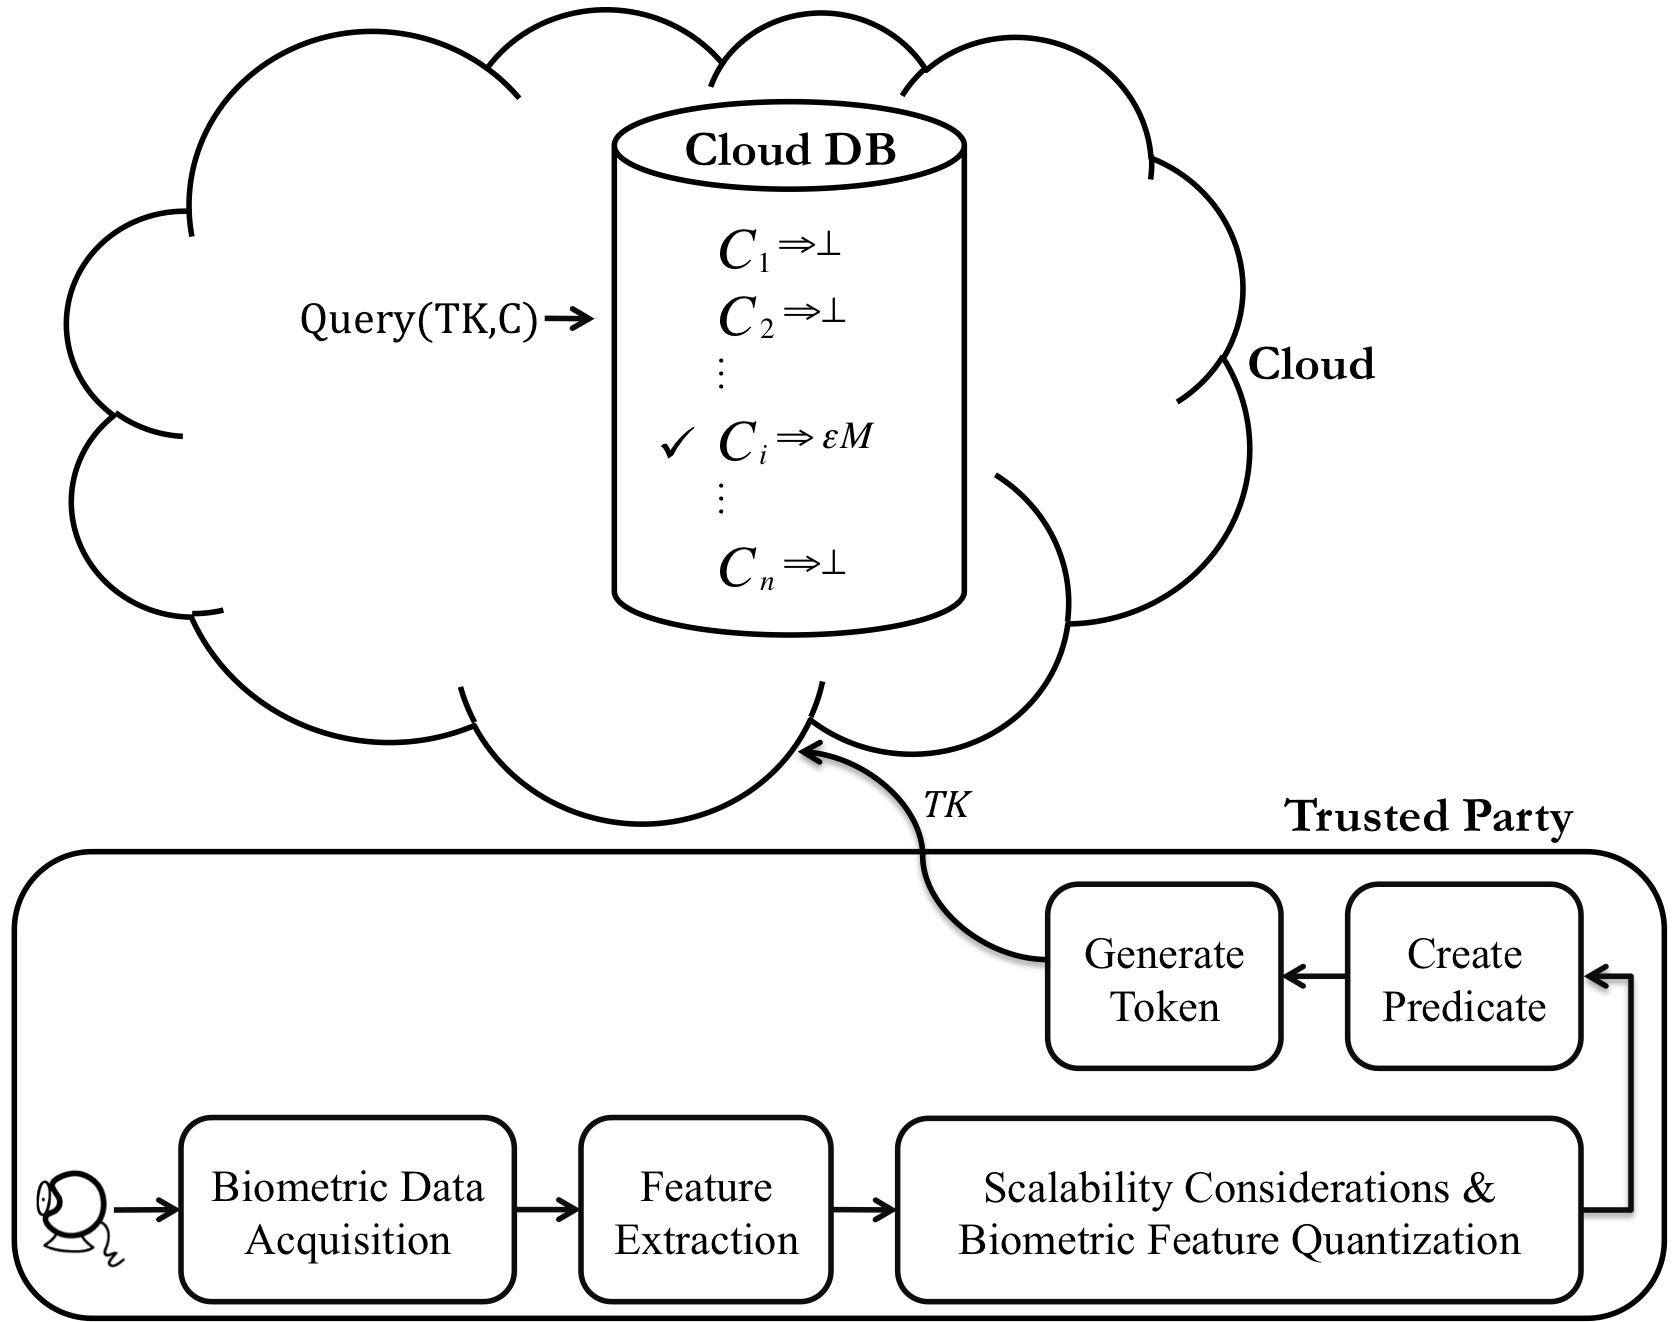
\includegraphics[width=0.6\textwidth]{./Figures/big-picture.png}
\caption{This is where the caption of the figure goes.}
\label{fig:big-picture}
\end{figure}



\section{Equations} \label{sec:equation}

Section \ref{sec:equation} is just an example to show how to insert inline and numbered equations. 

The inline equations has to be inserted between two dollar signs. Some examples are: $X^{\prime}$, or $Y^{\prime}$, or $S_{xy_{(r\times r)}}^{\prime}$. 

The numbered equations, on the other hand, need to be placed in an equation environment beginning and ending as below:
%
\begin{equation} \label{eq:1}
(U \Sigma^{-1/2})^T \, S_{xy}^{\prime} \, (V \Sigma^{-1/2}) = I \,,
\end{equation}
%
which is numbered as Eq. \ref{eq:1}.

Eq. \ref{eq:2} is an example of a multi-line equation:
\begin{equation} \begin{split} \label{eq:2}
G(x,y)=\frac{f^2}{\pi\gamma\eta} exp{\left(-\frac{x'^2+\gamma^2 y'^2}{2\sigma^2}\right)} exp{\left( j2\pi f x' + \phi \right)}     \\
x' = \;\;\; xcos\theta+ysin\theta    \\
y' = -xsin\theta+ycos\theta
\end{split} \end{equation}


\begin{table}[t]
\renewcommand{\arraystretch}{1.1}
\caption{This is where the caption of the table goes.}
\label{tab:runTime}
\centering
\footnotesize
\vspace{-0.1in}
\begin{tabular}{|l|c|}
\hline
Method				& 	Run Time (in milliseconds)\\
\hline\hline
Serial + PCA + KNN 		& 	19		\\
Serial + LDA + KNN 		& 	24		\\
Parallel + PCA + KNN 		& 	39		\\
Parallel + LDA + KNN 		& 	42		\\
PCA + CCA + KNN 		& 	19		\\
LDA + CCA + KNN 		& 	21		\\
JSRC 				& 	8406		\\
SMDL				&	7882		\\
DCA + KNN 			& 	19		\\
\hline
\end{tabular}
\vspace{-0.1in}
\end{table}




\vspace{0.2in}
\section{Section Title}\label{sec:foo}

This is an example to show how to insert sections in your chapter.



\vspace{0.2in}
\subsection{SubSection Title}\label{sec:bar}

This is an example of a sub-section.
Table \ref{tab:runTime} is just an example to show how to insert tables.



\vspace{0.2in}
\subsubsection{SubSubSection Title}

This is an example of a sub-sub-section, and another Table \ref{tab:wvu}.



\begin{table}[h]
\renewcommand{\arraystretch}{1.1}
\caption{Rank-1 recognition rates for multimodal fusion of face, ear and profile face biometrics in WVU database.}
\label{tab:wvu}
\centering
\footnotesize
\vspace{-0.1in}
\begin{tabular}{|l|c|c|c|}
\hline
\diagbox{Method}{Modality}	& Face+Ear		& Ear+Profile	& \begin{tabular}[x]{@{}c@{}}Face+Ear\\+Profile\end{tabular}	\\
\hline \hline
Serial + PCA + KNN		& $89.14 \pm 1.15$ 	& $89.46 \pm 1.13$	& $92.28 \pm 1.11$ 	\\
Serial + LDA + KNN		& $94.23 \pm 1.02$ 	& $95.14 \pm 1.20$	& $95.14 \pm 1.04$ 	\\
Parallel + PCA + KNN		& $90.71 \pm 2.05$ 	& $90.61 \pm 1.86$	& 	-		\\
Parallel + LDA + KNN		& $93.38 \pm 1.66$ 	& $93.13 \pm 1.67$	& 	-		\\
PCA + CCA/MCCA + KNN		& $94.10 \pm 0.87$ 	& $94.34 \pm 0.57$	& $97.74 \pm 0.54$ 	\\
LDA + CCA/MCCA + KNN		& $94.44 \pm 0.88$ 	& $94.89 \pm 0.54$	& $97.86 \pm 0.49$ 	\\
JSRC				& $96.20 \pm 0.52$	& $97.74 \pm 0.42$	& $98.74 \pm 0.32$	\\
SMDL				& $97.24 \pm 0.48$	& $97.97 \pm 0.42$	& $99.20 \pm 0.24$	\\
DCA/MDCA + KNN			& $98.56 \pm 0.15$ 	& $99.38 \pm 0.08$ 	& $99.85 \pm 0.03$  	\\
\hline
\end{tabular}
\end{table}
